\documentclass[11pt]{article}

\usepackage[margin=1in]{geometry}
\usepackage{amsmath,amssymb,amsthm}
\usepackage{tikz}
\usepackage{hyperref}

\theoremstyle{plain}
\newtheorem{theorem}{Theorem}[section]
\newtheorem{proposition}[theorem]{Proposition}
\newtheorem{corollary}[theorem]{Corollary}
\newtheorem{lemma}[theorem]{Lemma}
\theoremstyle{definition}
\newtheorem{definition}[theorem]{Definition}
\newtheorem{example}[theorem]{Example}
\theoremstyle{remark}
\newtheorem{remark}[theorem]{Remark}

\title{Why the Cauchy Problem for the Hamilton--Jacobi Equation\\
Generically Has No Global Solution:\\
Caustics Even in $H=p^2/2m+V(x)$}
\author{}
\date{\today}

\begin{document}
\maketitle

\begin{abstract}
\noindent
We give a self-contained, quantitative account of a fact that is well known to
specialists and routinely surprising on first encounter: the Cauchy
(initial value) problem for the time-dependent Hamilton--Jacobi equation
\[
\partial_t S(x,t) + H\big(x,\partial_x S(x,t)\big) = 0, \qquad S(x,0) = S_0(x),
\]
generically has \emph{no} solution that is smooth and single-valued for all
$t>0$ -- even when $H(x,p) = p^2/2m + V(x)$ is the simplest Hamiltonian in
classical mechanics. We rederive the method of characteristics, reduce the
question of global-in-time smooth solvability to the non-vanishing of a
Jacobian obeying a linear \emph{Jacobi equation}, and show that this
Jacobian generically vanishes in finite time. We then treat, in complete
elementary detail, the free particle and the harmonic oscillator: for the
latter we prove that \emph{every} $C^2$ initial phase $S_0$, however
gentle, produces a singularity by a universal, data-independent time
$t^\ast < \pi/\omega$, and we give the exact closed-form blow-up time. We
explain why this singularity is a geometric \emph{caustic} -- a fold of a
Lagrangian manifold -- rather than a genuine loss of information as in a
shock wave, and we discuss the two standard remedies: the multivalued
semiclassical (WKB/Maslov) continuation, and the single-valued
Crandall--Lions viscosity solution given by a Hopf--Lax-type variational
formula.
\end{abstract}

\tableofcontents

\section{Introduction}

In a first course, the Hamilton--Jacobi equation (HJE) is usually introduced as
a slightly baroque alternative to Hamilton's equations: separate variables,
find a complete integral, and the trajectories fall out for free. This leaves
the impression that the HJE is an evolution equation on the same footing as the
heat equation or the Schr\"odinger equation, so that prescribing
$S(x,0)=S_0(x)$ ought to determine $S(x,t)$ for all later times, in exact
analogy with how $\psi(x,0)$ determines $\psi(x,t)$ under Schr\"odinger
evolution.

This impression is false, and it fails already for the least exotic Hamiltonian
one can write down,
\begin{equation}
H(x,p) = \frac{p^2}{2m} + V(x),
\label{eq:H}
\end{equation}
with $V$ as smooth and as tame as one likes -- including $V\equiv 0$. The
purpose of this note is to make completely explicit, elementary, and
quantitative the precise sense in which the Cauchy problem for the HJE with
Hamiltonian \eqref{eq:H} cannot, generically, be posed for all time.

We will show the following.
\begin{itemize}
\item[(i)] A local-in-time smooth solution always exists
    (Section~\ref{sec:characteristics}), constructed by the method of
        characteristics, which reduces the first-order \emph{partial}
        differential equation to Hamilton's \emph{ordinary} differential
        equations.
\item[(ii)] Whether this local solution extends to a given later time $t$ is
    controlled entirely by the non-vanishing of a single scalar quantity
        $J(t,x_0)$ -- the Jacobian of the map ``initial position $\mapsto$
        position at time $t$'' -- which obeys a \emph{linear, second-order}
        ODE, the Jacobi equation (Section~\ref{sec:jacobi}).
\item[(iii)] For the free particle, $J$ blows down to zero in finite time
    unless the initial phase $S_0$ is convex; ``most'' data are not convex
        (Section~\ref{sec:free}).
\item[(iv)] For the harmonic oscillator -- arguably \emph{the} most elementary
    confining potential in physics -- $J$ vanishes in finite time for
        \emph{every} choice of $S_0$ whatsoever, with an explicit, universal
        bound on the blow-up time (Section~\ref{sec:sho}).
\item[(v)] The resulting singularity is not a defect of the method; it is a
    geometric \emph{caustic}, and we explain precisely what it is (a fold
        singularity of a Lagrangian submanifold under projection to
        configuration space) and what it is not (a shock wave, in the sense of
        a scalar conservation law) (Section~\ref{sec:geometry}).
\item[(vi)] We describe the two standard ways of continuing the solution past
    the singular time -- the multivalued semiclassical construction and the
        single-valued viscosity solution -- and note that both correspond to
        genuinely different, non-classical notions of ``solving'' the HJE
        (Section~\ref{sec:continuations}).
\end{itemize}

We stress at the outset why this is not a pathology of complicated potentials:
the source of the nonlinearity responsible for all of it is the kinetic term
$p^2/2m$ by itself. As we show in Section~\ref{sec:free}, the free particle
($V\equiv 0$) already exhibits finite-time breakdown for a generic initial
phase.

\begin{remark}
    Throughout, $S(x,t)$ denotes Hamilton's \emph{principal function}, the solution
    of the time-dependent HJE $\partial_tS + H(x,\partial_xS)=0$. This should
    not be confused with Hamilton's \emph{characteristic function} $W(x,E)$,
    which solves the time-independent equation $H(x,\partial_xW)=E$ and is used
    for separable, energy-conserving problems; the characteristic function is
    unproblematic to define (it is just a line integral of
    $p(x,E)=\pm\sqrt{2m(E-V(x))}$) and is not the subject of this paper. It is
    $S(x,t)$, the \emph{generator of the time-$t$ flow as a canonical
    transformation}, whose Cauchy problem is generically ill-posed for all
    time.
\end{remark}

\section{The Hamilton--Jacobi Cauchy problem}
\label{sec:setup}

Fix a mass $m>0$ and a potential $V\in C^k(\mathbb{R})$, $k\ge 2$, and let $H$
be as in \eqref{eq:H}. The Cauchy problem under discussion is: given 
$S_0 \in C^k(\mathbb{R})$, 
find $S\in C^1(\mathbb{R}\times[0,T))$, for as large a $T$ as
possible, solving
\begin{equation}
\partial_t S(x,t) + \frac{1}{2m}\big(\partial_x S(x,t)\big)^2 + V(x) = 0, \qquad S(x,0)=S_0(x).
\label{eq:HJE}
\end{equation}

Recall the mechanical meaning of $S$: if $S$ solves \eqref{eq:HJE}, then the
vector field $p(x,t):=\partial_xS(x,t)$ is a \emph{momentum field} -- at each
point $x$ and time $t$, it prescribes the momentum of the classical trajectory
passing through $x$ at time $t$ -- and $S(x,t)$ equals the classical action
accumulated along that trajectory since $t=0$,
\begin{equation}
S(x,t) = S_0(x_0) + \int_0^t L\big(x(\tau),\dot x(\tau)\big)\,d\tau, \qquad L(x,\dot x)=\tfrac12 m\dot x^2 - V(x),
\label{eq:action}
\end{equation}
where $x(\cdot)$ is the classical trajectory with $x(0)=x_0$ and $x(t)=x$.
Equation \eqref{eq:action} is not an assumption; it is a theorem, proved in
Section~\ref{sec:characteristics} below.

The question we address is exactly: for which $T$ does there exist a single
$C^1$ function on $\mathbb{R}\times[0,T)$ (or on some fixed spatial domain of
interest, times $[0,T)$) satisfying \eqref{eq:HJE} pointwise? We will see that
the honest answer, for essentially every choice of $V$ and $S_0$, is:
\emph{only for $T$ up to some finite $t^\ast$}, no matter how smooth $V$ and
$S_0$ are.

\section{Characteristics: the PDE becomes an ODE}
\label{sec:characteristics}

\begin{proposition}[Characteristics of the HJE]
\label{prop:characteristics}
Suppose $S\in C^2(\mathbb{R}\times[0,T))$ solves \eqref{eq:HJE}. Fix
    $x_0\in\mathbb{R}$ and let $x(\cdot)$ solve the ordinary differential
    equation
\[
\dot x(t) = \partial_pH\big(x(t),\partial_xS(x(t),t)\big) =
    \frac{1}{m}\partial_xS(x(t),t), \qquad x(0)=x_0,
\]
for as long as this makes sense. Set $p(t):=\partial_xS(x(t),t)$ 
    and $\sigma(t):=S(x(t),t)$. Then
\begin{equation}
\dot x = \frac{p}{m}, \qquad \dot p = -V'(x), 
    \qquad \dot\sigma = p\dot x - H(x,p) = L(x,\dot x).
\label{eq:hameqs}
\end{equation}
That is, $(x(t),p(t))$ is a solution of Hamilton's equations, and $\sigma$ is
    the classical action accumulated along it.
\end{proposition}

\begin{proof}
Differentiate the defining relation for $p$ along the curve:
\[
\dot p = \frac{d}{dt}\,\partial_xS(x(t),t) = \partial_t\partial_xS +
    \dot x\,\partial_x^2 S.
\]
Differentiate the PDE \eqref{eq:HJE} itself with respect to $x$:
\[
\partial_x\partial_tS + V'(x) + \frac{1}{m}\partial_xS\,\partial_x^2S = 0
\quad\Longrightarrow\quad
\partial_t\partial_xS = -V'(x) - \dot x\,\partial_x^2S,
\]
where we used $\dot x = \frac1m\partial_xS(x(t),t)=\frac1m p$. Substituting,
\[
\dot p = \big(-V'(x)-\dot x\,\partial_x^2S\big) + \dot x\,\partial_x^2S = -V'(x),
\]
which is the second equation in \eqref{eq:hameqs}. Finally,
\[
\dot\sigma = \frac{d}{dt}S(x(t),t) = \partial_tS + \dot x\,\partial_xS = -H(x,p) + \dot x\,p = p\dot x - H(x,p),
\]
using \eqref{eq:HJE} for $\partial_tS$. Since $H(x,p)=p^2/2m+V(x)$ is the Legendre transform of $L(x,\dot x)=\tfrac12m\dot x^2-V(x)$ with $p=m\dot x$, and $\dot x=p/m$ by construction, we have $p\dot x-H(x,p)=L(x,\dot x)$ exactly.
\end{proof}

Proposition~\ref{prop:characteristics} converts the search for $S$ into the
elementary task of solving Hamilton's equations, an autonomous system of ODEs
with smooth (as smooth as $V$) right-hand side, hence with a smooth, locally
unique flow. Denote by $(x(t;x_0),p(t;x_0))$ the solution with
\[
x(0;x_0)=x_0, \qquad p(0;x_0)=S_0'(x_0),
\]
and define the \textbf{stretching factor}
\begin{equation}
J(t,x_0) := \frac{\partial x}{\partial x_0}(t;x_0).
\label{eq:Jdef}
\end{equation}
By construction $J(0,x_0)=1$ for every $x_0$.

\begin{theorem}[Local solvability, and its limit]
\label{thm:local}
Let $V,S_0\in C^k(\mathbb{R})$, $k\ge 2$. Fix $x_0$, and let
\begin{equation}
t^\ast(x_0) := \sup\{\,T>0 : J(t,x_0)\ne 0 \text{ for all } t\in[0,T)\,\} \ \in (0,\infty].
\label{eq:tstar}
\end{equation}
Then for every $T<t^\ast(x_0)$ there is an interval $I\ni x_0$ and a
    neighborhood of $\{x(t;x_0): t\in[0,T]\}$ on which $x_0\mapsto x(t;x_0)$
    is, for each fixed $t\le T$, a $C^{k-1}$ diffeomorphism from $I$ onto its
    image; writing $x_0(x,t)$ for its inverse, the function
\[
S(x,t) := S_0\big(x_0(x,t)\big) + \int_0^t L\Big(x\big(\tau;x_0(x,t)\big),
    \dot x\big(\tau;x_0(x,t)\big)\Big)\,d\tau
\]
is the unique $C^1$ solution of \eqref{eq:HJE} on that neighborhood, for
    $t\in[0,T]$. Conversely, no single-valued $C^1$ function can solve
    \eqref{eq:HJE} in any neighborhood of
    $\big(x(t^\ast(x_0);x_0),t^\ast(x_0)\big)$ extending past $t=t^\ast(x_0)$,
    if $x_0\mapsto x(t;x_0)$ fails to be injective near $x_0$ for $t$ slightly
    larger than $t^\ast(x_0)$ -- which is the generic situation.
\end{theorem}

\begin{proof}[Proof sketch]
Existence for $t<t^\ast(x_0)$: since $J(0,x_0)=1\ne0$ and $J$ is continuous,
    $J\ne0$ on $[0,T]$ for $T<t^\ast(x_0)$; by the inverse function theorem,
    $x_0\mapsto x(t;x_0)$ is then a local diffeomorphism, uniformly for
    $t\in[0,T]$, on some interval $I$. That the resulting $S(x,t)$ solves
    \eqref{eq:HJE} is a direct (if slightly tedious) computation using
    Proposition~\ref{prop:characteristics} in reverse, and is the classical
    content of the method of characteristics for first-order PDEs; see
    Courant--Hilbert \cite{CourantHilbert} or Evans \cite{Evans}, \S3.2--3.3.

Uniqueness, and the impossibility of continuation: if $\tilde S$ is \emph{any}
    $C^1$ solution of \eqref{eq:HJE} near a point $(x,t)$, set $\tilde
    p(x,t):=\partial_x\tilde S(x,t)$ and let $\tilde x(\cdot)$ solve
    $\dot{\tilde x}=\tilde p(\tilde x,\cdot)/m$ through $(x,t)$. Running
    Proposition~\ref{prop:characteristics}'s argument backward in time shows
    $(\tilde x(\cdot),\tilde p(\tilde x(\cdot),\cdot))$ satisfies Hamilton's
    equations; by uniqueness of solutions of ODEs with Lipschitz right-hand
    side, this trajectory must coincide with $(x(\cdot;x_0),p(\cdot;x_0))$ for
    the appropriate $x_0$. Hence \emph{every} $C^1$ solution, wherever defined,
    must agree with the characteristic construction. If, at time
    $t>t^\ast(x_0)$, two distinct characteristics $x_0\ne x_0'$ satisfy
    $x(t;x_0)=x(t;x_0')=x$, then any $C^1$ solution would be forced to satisfy
    $\partial_x\tilde S(x,t) = p(t;x_0)$ \emph{and} $\partial_x\tilde
    S(x,t)=p(t;x_0')$ simultaneously; if $p(t;x_0)\ne p(t;x_0')$ (the generic
    case at a simple fold), this is a contradiction, so no such $\tilde S$
    exists.
\end{proof}

Theorem~\ref{thm:local} reduces everything to the study of $J(t,x_0)$, i.e., to
a linear second-order ODE, which we derive next.

\section{The Jacobi equation and the breakdown criterion}
\label{sec:jacobi}

Differentiate Hamilton's equations \eqref{eq:hameqs} with respect to the label
$x_0$. Writing $J=\partial_{x_0}x$ and $K=\partial_{x_0}p$,
\[
\dot J = \frac{1}{m}K, \qquad \dot K = -V''\big(x(t;x_0)\big)\,J,
\]
and hence
\begin{equation}
\ddot J(t,x_0) + \frac{1}{m}V''\big(x(t;x_0)\big)\,J(t,x_0) = 0, \qquad J(0,x_0)=1, \quad \dot J(0,x_0) = \frac{S_0''(x_0)}{m}.
\label{eq:jacobi}
\end{equation}
This is precisely the \emph{Jacobi equation} (Jacobi accessory equation) of the
classical calculus of variations, governing the second variation of the action
along the extremal $x(\cdot;x_0)$; see Arnold \cite{Arnold}, \S22--23, or
Milnor \cite{Milnor}, \S15. A zero of $J$ is, by definition, a
\textbf{conjugate point} along the trajectory. So Theorem~\ref{thm:local} says:

\begin{center}
\emph{the smooth HJE solution breaks down at exactly the first conjugate point.}
\end{center}

This is not a coincidence but the same fact seen from two sides: a conjugate
point is exactly the point where the trajectory $x(\cdot;x_0)$ stops being even
a local minimizer of the action (Jacobi's necessary condition), and it is
exactly the point where the family of nearby trajectories, which the generating
function $S$ is supposed to organize into a single-valued momentum field,
starts to overlap.

\begin{remark}
Up to normalization, $J(t,x_0)^{-1}$ is (the one-dimensional case of) the Van
    Vleck--Morette determinant that controls the amplitude of the semiclassical
    (WKB) approximation to the quantum propagator. Its vanishing is precisely
    the condition under which the leading-order WKB amplitude diverges,
    signalling the breakdown of the naive semiclassical approximation and the
    need for Airy-function (uniform) corrections near the caustic; see
    Maslov--Fedoriuk \cite{MaslovFedoriuk} and Guillemin--Sternberg
    \cite{GuilleminSternberg}.
\end{remark}

We now solve \eqref{eq:jacobi} explicitly for the two simplest potentials there are.

\section{Two boring examples}
\label{sec:examples}

\subsection{The free particle}
\label{sec:free}

Take $V\equiv0$. Then $V''\equiv0$ and \eqref{eq:jacobi} integrates trivially:
\begin{equation}
J(t,x_0) = 1 + \frac{S_0''(x_0)}{m}\,t.
\label{eq:Jfree}
\end{equation}

\begin{proposition}
\label{prop:free}
For the free particle, the classical HJE solution starting from $x_0$ exists
    for all $t>0$ if and only if $S_0''(x_0)\ge 0$. If $S_0''(x_0)<0$, it
    breaks down at the finite time
\[
t^\ast(x_0) = -\frac{m}{S_0''(x_0)}.
\]
\end{proposition}

The condition $S_0''\ge0$ everywhere means $S_0$ is convex: the initial
momentum field $p_0(x)=S_0'(x)$ is non-decreasing, so nearby particles are, at
worst, drifting apart or moving in parallel -- never converging. This is a very
restrictive condition (violated, for instance, on an open dense set of $C^2$
functions in any reasonable topology): the mere presence of one convergent
region in the initial data destroys global existence.

\begin{example}[A lens]
Take $S_0(x) = -\dfrac{m}{2\tau}x^2$ for some $\tau>0$, i.e., an initial
    momentum field $p_0(x)=-\frac{m}{\tau}x$ pointing uniformly toward the
    origin -- literally the phase profile of a converging lens. Every
    characteristic is a straight line,
\[
x(t;x_0) = x_0\Big(1-\frac{t}{\tau}\Big),
\]
and \emph{all of them meet at the single point $x=0$ at time $t=\tau$}: a
    perfect focus, formed instantly out of the most boring possible dynamics
    (free motion) acting on smooth, everywhere-defined data. See
    Figure~\ref{fig:focus}.
\end{example}

\begin{figure}[h]
\centering
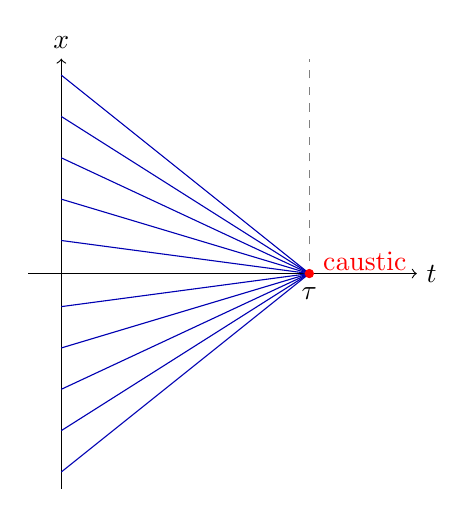
\begin{tikzpicture}[scale=1.05]
\draw[->] (-0.4,0) -- (4.3,0) node[right] {$t$};
\draw[->] (0,-2.6) -- (0,2.6) node[above] {$x$};
\draw[dashed,gray] (3,-0.05) -- (3,2.6);
\node[below] at (3,-0.05) {$\tau$};
\foreach \xa in {-2.4,-1.9,-1.4,-0.9,-0.4,0.4,0.9,1.4,1.9,2.4}{
  \draw[thin,blue!70!black] (0,\xa) -- (3,0);
}
\filldraw[red] (3,0) circle (1.4pt);
\node[right,red] at (3.05,0.15) {caustic};
\end{tikzpicture}
\caption{Characteristics $x(t;x_0)=x_0(1-t/\tau)$ of the free particle with
    converging initial phase $S_0(x)=-\frac{m}{2\tau}x^2$. Every trajectory,
    however far from the origin it starts, reaches $x=0$ at the same instant
    $t=\tau$: a caustic forms in finite time even though $V\equiv0$.}
\label{fig:focus}
\end{figure}

\subsection{The harmonic oscillator}
\label{sec:sho}

Take $V(x)=\tfrac12 m\omega^2x^2$, so $V''\equiv m\omega^2$ is constant, and
\eqref{eq:jacobi} becomes the harmonic-oscillator equation itself,
\[
\ddot J + \omega^2 J = 0, \qquad J(0,x_0)=1,\quad \dot J(0,x_0)=\frac{S_0''(x_0)}{m},
\]
with exact solution
\begin{equation}
J(t,x_0) = \cos\omega t + \frac{S_0''(x_0)}{m\omega}\sin\omega t.
\label{eq:Jsho}
\end{equation}

\begin{theorem}[Universal breakdown]
\label{thm:sho}
For the harmonic oscillator, for \emph{every} $S_0\in C^2(\mathbb{R})$ and
    \emph{every} $x_0\in\mathbb{R}$, the classical HJE solution starting from
    $x_0$ breaks down at the finite time
\begin{equation}
t^\ast(x_0) = \frac{1}{\omega}\left[\frac{\pi}{2} + \arctan\!\left(\frac{S_0''(x_0)}{m\omega}\right)\right] \ \in\ \Big(0,\ \frac{\pi}{\omega}\Big).
\label{eq:tstarsho}
\end{equation}
In particular $t^\ast(x_0) < \pi/\omega$ uniformly in $x_0$ and in $S_0$: no choice of smooth initial phase, however gentle, avoids a caustic within one half-period of the oscillator.
\end{theorem}

\begin{proof}
Write $A=1$, $B=S_0''(x_0)/(m\omega)$, so $J(t,x_0)=A\cos\omega t+B\sin\omega t
    = R\cos(\omega t-\phi)$ with $R=\sqrt{A^2+B^2}>0$ and
    $\phi=\arctan(B/A)=\arctan B\in(-\tfrac\pi2,\tfrac\pi2)$ (the branch is
    fixed by $A=1>0$). The zeros of $J$ are at $\omega t-\phi=\tfrac\pi2+k\pi$,
    $k\in\mathbb Z$, i.e. $t=(\phi+\tfrac\pi2+k\pi)/\omega$. Since
    $\phi\in(-\tfrac\pi2,\tfrac\pi2)$, the value at $k=0$ lies in
    $(0,\pi/\omega)$ and is manifestly the smallest positive root (the $k=-1$
    root is negative). This proves \eqref{eq:tstarsho}.
\end{proof}

Sanity checks on \eqref{eq:tstarsho}: if $S_0''(x_0)=0$ (locally ``flat''
data), $t^\ast=\pi/(2\omega)$, a quarter period. As $S_0''(x_0)\to+\infty$
(strongly diverging data), $t^\ast\to\pi/\omega$ but never reaches it. As
$S_0''(x_0)\to-\infty$ (strongly focusing data), $t^\ast\to0^+$: an
already-converging beam focuses almost instantly, exactly as one would guess.
What Theorem~\ref{thm:sho} adds is that \emph{even the most favorable, most
divergent possible data cannot postpone the caustic past $t=\pi/\omega$}. This
finite, data-independent interval between conjugate points is a classical fact
about the harmonic oscillator (Arnold \cite{Arnold}, \S23) and is the
mechanical origin of the Maslov index increasing by one unit every half-period
in the semiclassical (Bohr--Sommerfeld--Maslov) quantization of the oscillator.

\subsection{General uniformly convex potentials}

Theorem~\ref{thm:sho} is not special to the exactly quadratic potential; it is
the model case of a much more general comparison principle.

\begin{theorem}
\label{thm:sturm}
Suppose $V\in C^2(\mathbb{R})$ satisfies $V''(x)\ge m\omega^2$ for all
    $x\in\mathbb{R}$, for some $\omega>0$. Then for every $S_0\in
    C^2(\mathbb{R})$ and every $x_0\in\mathbb{R}$,
\[
t^\ast(x_0) < \frac{\pi}{\omega}.
\]
\end{theorem}

\begin{proof}
Along the trajectory, $q(t):=V''\big(x(t;x_0)\big)/m \ge \omega^2$ for all $t$,
    so $J$ solves $\ddot J + q(t)J=0$ with $J(0,x_0)=1\ne0$. Let
    $y(t)=\sin\omega t$, which solves $\ddot y+\omega^2y=0$ and has consecutive
    zeros at $t=0$ and $t=\pi/\omega$, with $y\ne0$ in between. By the Sturm
    comparison theorem (see, e.g., Coddington--Levinson
    \cite{CoddingtonLevinson}, Ch.~8) applied to $\ddot J+qJ=0$ against $\ddot
    y+\omega^2y=0$ with $q\ge\omega^2$, $J$ must vanish somewhere in
    $(0,\pi/\omega)$ unless $J$ is a constant multiple of $y$ -- impossible
    here since $J(0,x_0)=1\ne 0=y(0)$.
\end{proof}

\begin{remark}
Theorem~\ref{thm:sturm} is the exact one-dimensional mechanical analogue of the
    Rauch comparison theorem in Riemannian geometry (see do Carmo
    \cite{doCarmo}), in which $V''$ plays the role of sectional curvature: a
    lower bound on curvature (here, on the ``restoring strength'' of the
    potential) forces conjugate points to appear within a bounded distance --
    the mechanical cousin of the Bonnet--Myers theorem. Convexity of $V$ is
    what does the damage; potentials that are flat or concave ($V''\le0$)
    behave more like the free particle of Section~\ref{sec:free}, where global
    existence is possible but only for a non-generic (convex) subset of initial
    data.
\end{remark}

\section{What the singularity actually is: caustics, not shocks}
\label{sec:geometry}

It is tempting, on seeing \eqref{eq:jacobi} blow down to zero, to think of this
as a shock wave forming out of smooth data, as in Burgers' equation. The
analogy is real but must be handled carefully, because taken too literally it
suggests the wrong physical resolution.

Differentiating \eqref{eq:HJE} once in $x$ and writing $p=\partial_xS$ gives the momentum-field equation
\begin{equation}
\partial_tp + \frac{1}{m}\,p\,\partial_xp = -V'(x).
\label{eq:burgers}
\end{equation}
For $V\equiv0$ this is exactly the inviscid Burgers equation for $u=p/m$, whose
characteristics are the same straight lines drawn in Figure~\ref{fig:focus}. So
far the analogy is exact. But there is a crucial difference in what the
crossing of characteristics \emph{means}.

Consider the full phase-space curve
\[
\Lambda_t := \big\{(x(t;x_0),p(t;x_0)) : x_0\in\mathbb{R}\big\} \subset \mathbb{R}^2.
\]
Because the Hamiltonian flow generated by \eqref{eq:H} is, for the potentials
considered here, a complete flow of smooth diffeomorphisms of the phase plane
for all $t\in\mathbb{R}$, the curve $\Lambda_t$ is perfectly smooth for
\emph{every} $t$ -- nothing in phase space ever collides, merges, or loses
information: this is just Liouville's theorem together with uniqueness of
solutions of Hamilton's equations. What happens at $t=t^\ast(x_0)$ is entirely
a statement about the \emph{projection}
\[
\pi:\Lambda_t\to\mathbb{R}_x, \qquad (x,p)\mapsto x,
\]
whose derivative along $\Lambda_t$ at the point labelled by $x_0$ is exactly
$J(t,x_0)$. At $t=t^\ast(x_0)$, $\pi$ develops a critical point: $\Lambda_t$ is
momentarily tangent to the fibre direction there. This is a \emph{fold}, in the
sense of Whitney and Thom's theory of singularities of smooth maps (see Arnold
\cite{ArnoldCatastrophe} for an accessible account); immediately afterward,
$\pi$ is locally two-to-one, and two distinct sheets of $\Lambda_t$ -- two
distinct momenta -- sit over the same $x$. This is precisely a \emph{caustic}
in the sense of geometric optics: the bright curve on the floor of a swimming
pool, the cusp of a rainbow, the focal point of a lens in
Figure~\ref{fig:focus}. Rays (here, classical trajectories) do not disappear or
merge at a caustic; they simply cross, and go on to occupy the same point in
configuration space while carrying different momenta.

This is fundamentally different from a genuine shock in a scalar conservation
law, such as \eqref{eq:burgers} interpreted on its own as an evolution equation
for $p$ with, say, an entropy condition imposed to select a unique
discontinuous weak solution. That construction is appropriate for a dissipative
medium -- pressureless, sticky ``dust'' in which colliding particles merge and
information is genuinely lost, enforcing the Rankine--Hugoniot / Oleinik
entropy condition. It is not appropriate for the actual, collisionless
mechanical system \eqref{eq:hameqs} describes, in which trajectories pass
through one another. The two constructions coincide as pieces of formal
mathematics (the Lax--Oleinik entropy solution of \eqref{eq:burgers} is
literally $\partial_x$ of the Crandall--Lions viscosity solution of
\eqref{eq:HJE}, discussed in Section~\ref{sec:continuations}), but they answer
different physical questions. This distinction is exactly the one drawn, in a
cosmological setting, between the ``adhesion approximation'' (dust that sticks
upon crossing, described by the entropy solution) and the true collisionless
dynamics of the Zel'dovich approximation to large-scale structure formation, in
which multiple streams of matter coexist after crossing and form a genuinely
multivalued velocity field; see Zel'dovich \cite{Zeldovich}.

\section{Continuations past \texorpdfstring{$t^\ast$}{t*}}
\label{sec:continuations}

Given that no single-valued classical solution survives past the first caustic,
there are two standard, and genuinely different, ways to say something about
$t>t^\ast$.

\subsection{Multivalued continuation: the semiclassical picture}

The honest object that continues smoothly through the caustic is not $S(x,t)$
but the Lagrangian curve $\Lambda_t$ itself, which remains smooth for all time.
Near a fold, $\Lambda_t$ is more naturally parametrized by $p$ (or by
arclength) than by $x$, and the correct statement of ``the solution'' becomes:
locally, finitely many smooth branches $S_1(x,t),S_2(x,t),\dots$, one for each
sheet of $\Lambda_t$ lying over $x$.

This is exactly what happens, one order more precisely, in the semiclassical
(WKB) approximation to the Schr\"odinger equation. Substituting
$\psi(x,t)\approx A(x,t)e^{iS(x,t)/\hbar}$ into the Schr\"odinger equation and
expanding in powers of $\hbar$ produces \eqref{eq:HJE} at leading order and a
transport equation for $A$ at the next order, with $A\propto |J|^{-1/2}$; the
WKB amplitude literally diverges at the caustic, exactly where $J=0$. The
correct continuation is a coherent sum over the branches, each carrying an
extra phase $-i\pi\mu_j/2$ where $\mu_j$ (the Maslov index of that branch)
counts the conjugate points crossed so far; near the caustic itself, this
asymptotic sum must be replaced by an Airy-function uniform approximation. See
Maslov--Fedoriuk \cite{MaslovFedoriuk}, Guillemin--Sternberg
\cite{GuilleminSternberg}, and Berry--Upstill \cite{BerryUpstill} for the full
theory of these ``catastrophe optics'' corrections.

\subsection{Single-valued continuation: viscosity solutions}
\label{sec:viscosity}

Alternatively, one can insist on a single-valued function of $(x,t)$ defined
for \emph{all} time, at the cost of giving up smoothness. Define
\begin{equation}
S(x,t) \ :=\ \inf\Big\{\, S_0\big(\gamma(0)\big) + \int_0^tL\big(\gamma(\tau),\dot\gamma(\tau)\big)\,d\tau \ :\ \gamma \text{ absolutely continuous}, \ \gamma(t)=x \,\Big\},
\label{eq:hopflax}
\end{equation}
minimizing the total ``cost'' over \emph{all} paths ending at $x$ at time $t$,
with free initial point weighted by $S_0$. Because $L(x,\dot x)=\tfrac12m\dot
x^2-V(x)$ is strictly convex and superlinear in $\dot x$, this variational
problem is well posed for reasonable $V$ (e.g. bounded below, as for both
examples above), and \eqref{eq:hopflax} defines the unique \emph{viscosity
solution} of the Cauchy problem \eqref{eq:HJE}, in the sense of Crandall and
Lions \cite{CrandallLions}, for all $t\ge 0$ -- see Evans \cite{Evans}, Ch.~10,
or Fathi \cite{Fathi} for the Lagrangian (weak KAM) formulation of
\eqref{eq:hopflax}. (When $V$ is constant, minimizing paths are straight lines
and \eqref{eq:hopflax} reduces to the familiar Hopf--Lax formula.)

This $S$ agrees with the classical smooth solution of Theorem~\ref{thm:local}
for $t<t^\ast$, but for $t\ge t^\ast$ it typically develops a genuine kink -- a
jump in $\partial_xS$ -- exactly where two or more competing paths tie for the
minimum in \eqref{eq:hopflax}. In other words, \eqref{eq:hopflax} \emph{can} be
solved globally in time, but only by (i) discarding all but the single
\emph{minimal-action} branch at each point -- throwing away the very
trajectories whose mutual interference is physically encoded in the multivalued
WKB picture -- and (ii) accepting a solution that is merely Lipschitz, not
$C^1$, and therefore no longer ``the'' generating function of a canonical
transformation in the sense classical mechanics requires. This is the precise,
sharp form of the opening claim: a global solution in the classical
(single-sheeted, $C^1$) sense generically does not exist, and neither of the
two standard substitutes -- the multivalued semiclassical one or the
single-valued viscosity one -- is that classical solution; each recovers it
only for $t<t^\ast$ and replaces it with something structurally different
afterward.

\section{Discussion and conclusion}

The point of working out the free particle and the harmonic oscillator in such
elementary detail is to make it impossible to blame the phenomenon on some
contrived feature of $V(x)$. The free particle shows that the quadratic kinetic
term \emph{by itself} is enough to produce finite-time breakdown, for any
initial phase with a single region of concavity. The harmonic oscillator shows
that once any amount of convexity is added to $V$, breakdown becomes not merely
generic but \emph{unconditional}: literally no choice of $C^2$ initial data
survives past $t=\pi/\omega$. Between these two examples lies essentially every
problem discussed in an introductory mechanics course.

It is worth closing with the observation that this whole difficulty is a purely
classical artifact, absent from the parent theory. The HJE \eqref{eq:HJE} is
recovered from the Schr\"odinger equation for $\psi=Ae^{iS/\hbar}$ at leading
order in $\hbar$; the linear Schr\"odinger equation itself has a perfectly
well-posed, globally-in-time, unitary Cauchy problem for the same $H$. The
finite-time singularity of the classical theory is not a sign that something is
wrong with mechanics; it is a sign that the eikonal (leading-order,
$\hbar\to0$) approximation to a wave equation must generically develop
caustics, exactly as it does in ordinary geometric optics, and that resolving
them -- whether by keeping all interfering branches (semiclassical
continuation) or by passing to the variational, minimal-action solution
(viscosity continuation) -- requires input beyond the bare Cauchy data $S_0$.
What cannot be done, for essentially any $V$ and essentially any $S_0$, is what
a first encounter with the equation suggests should be routine: solve the
Cauchy problem once, classically, and be done with it for all time.

\begin{thebibliography}{99}

\bibitem{Arnold} V.~I.~Arnold, \emph{Mathematical Methods of Classical
    Mechanics}, 2nd ed., Graduate Texts in Mathematics 60, Springer, 1989.

\bibitem{ArnoldCatastrophe} V.~I.~Arnold, \emph{Catastrophe Theory}, 3rd ed., Springer, 1992.

\bibitem{BerryUpstill} M.~V.~Berry and C.~Upstill, \emph{Catastrophe optics:
    morphologies of caustics and their diffraction patterns}, in Progress in
        Optics XVIII, ed.\ E.\ Wolf, North-Holland, 1980, pp.~257--346.

\bibitem{CoddingtonLevinson} E.~A.~Coddington and N.~Levinson, \emph{Theory of
    Ordinary Differential Equations}, McGraw-Hill, 1955.

\bibitem{CourantHilbert} R.~Courant and D.~Hilbert, \emph{Methods of
    Mathematical Physics}, Vol.~II: Partial Differential Equations, Wiley,
        1962.

\bibitem{CrandallLions} M.~G.~Crandall and P.-L.~Lions, \emph{Viscosity
    solutions of Hamilton--Jacobi equations}, Trans.\ Amer.\ Math.\ Soc.\
        \textbf{277} (1983), 1--42.

\bibitem{doCarmo} M.~do~Carmo, \emph{Riemannian Geometry}, Birkh\"auser, 1992.

\bibitem{Evans} L.~C.~Evans, \emph{Partial Differential Equations}, 2nd ed.,
    Graduate Studies in Mathematics 19, American Mathematical Society, 2010.

\bibitem{Fathi} A.~Fathi, \emph{Weak KAM Theorem in Lagrangian Dynamics},
    Cambridge Studies in Advanced Mathematics, Cambridge University Press.

\bibitem{GuilleminSternberg} V.~Guillemin and S.~Sternberg, \emph{Geometric
    Asymptotics}, Mathematical Surveys 14, American Mathematical Society, 1977.

\bibitem{MaslovFedoriuk} V.~P.~Maslov and M.~V.~Fedoriuk, \emph{Semi-Classical
    Approximation in Quantum Mechanics}, Reidel, 1981.

\bibitem{Milnor} J.~Milnor, \emph{Morse Theory}, Annals of Mathematics Studies
    51, Princeton University Press, 1963.

\bibitem{Zeldovich} Ya.~B.~Zel'dovich, \emph{Gravitational instability: an
    approximate theory for large density perturbations}, Astronomy \&
        Astrophysics \textbf{5} (1970), 84--89.

\end{thebibliography}

\end{document}
